Nella fase di progettazione del gioco è stato deciso di implementare un gioco a quiz, in cui l'utente muovendo gli occhi avrebbe selezionato la risposta desiderata per la domanda sottoposta.

A tal proposito si è deciso di far riferimento al servizio OpentDB\cite{opentdb} (\textit{Open Trivia DB}) da cui tramite richieste $HTTP$ vengono acquisite 10 domande per iterazione in formato $JSON$. Successivamente vengono estratte solo le domande con quattro risposte possibili e mostrate a video i quesiti in modo sequenziale.

Il gioco in background abilita la fotocamera frontale e in tempo reale inizia il tracciamento degli occhi. Quando il tracciamento ha successo a video viene mostrato un cerchio rosso che rappresenta la posizione degli occhi. Muovendo gli occhi, e quindi il cerchio, su una risposta la si conferma. Se la risposta data è corretta il gioco mostrerà un'altra domanda fino a quando l'utente non sceglie di terminare il gioco.

\begin{figure}[htbp]
    \centering
    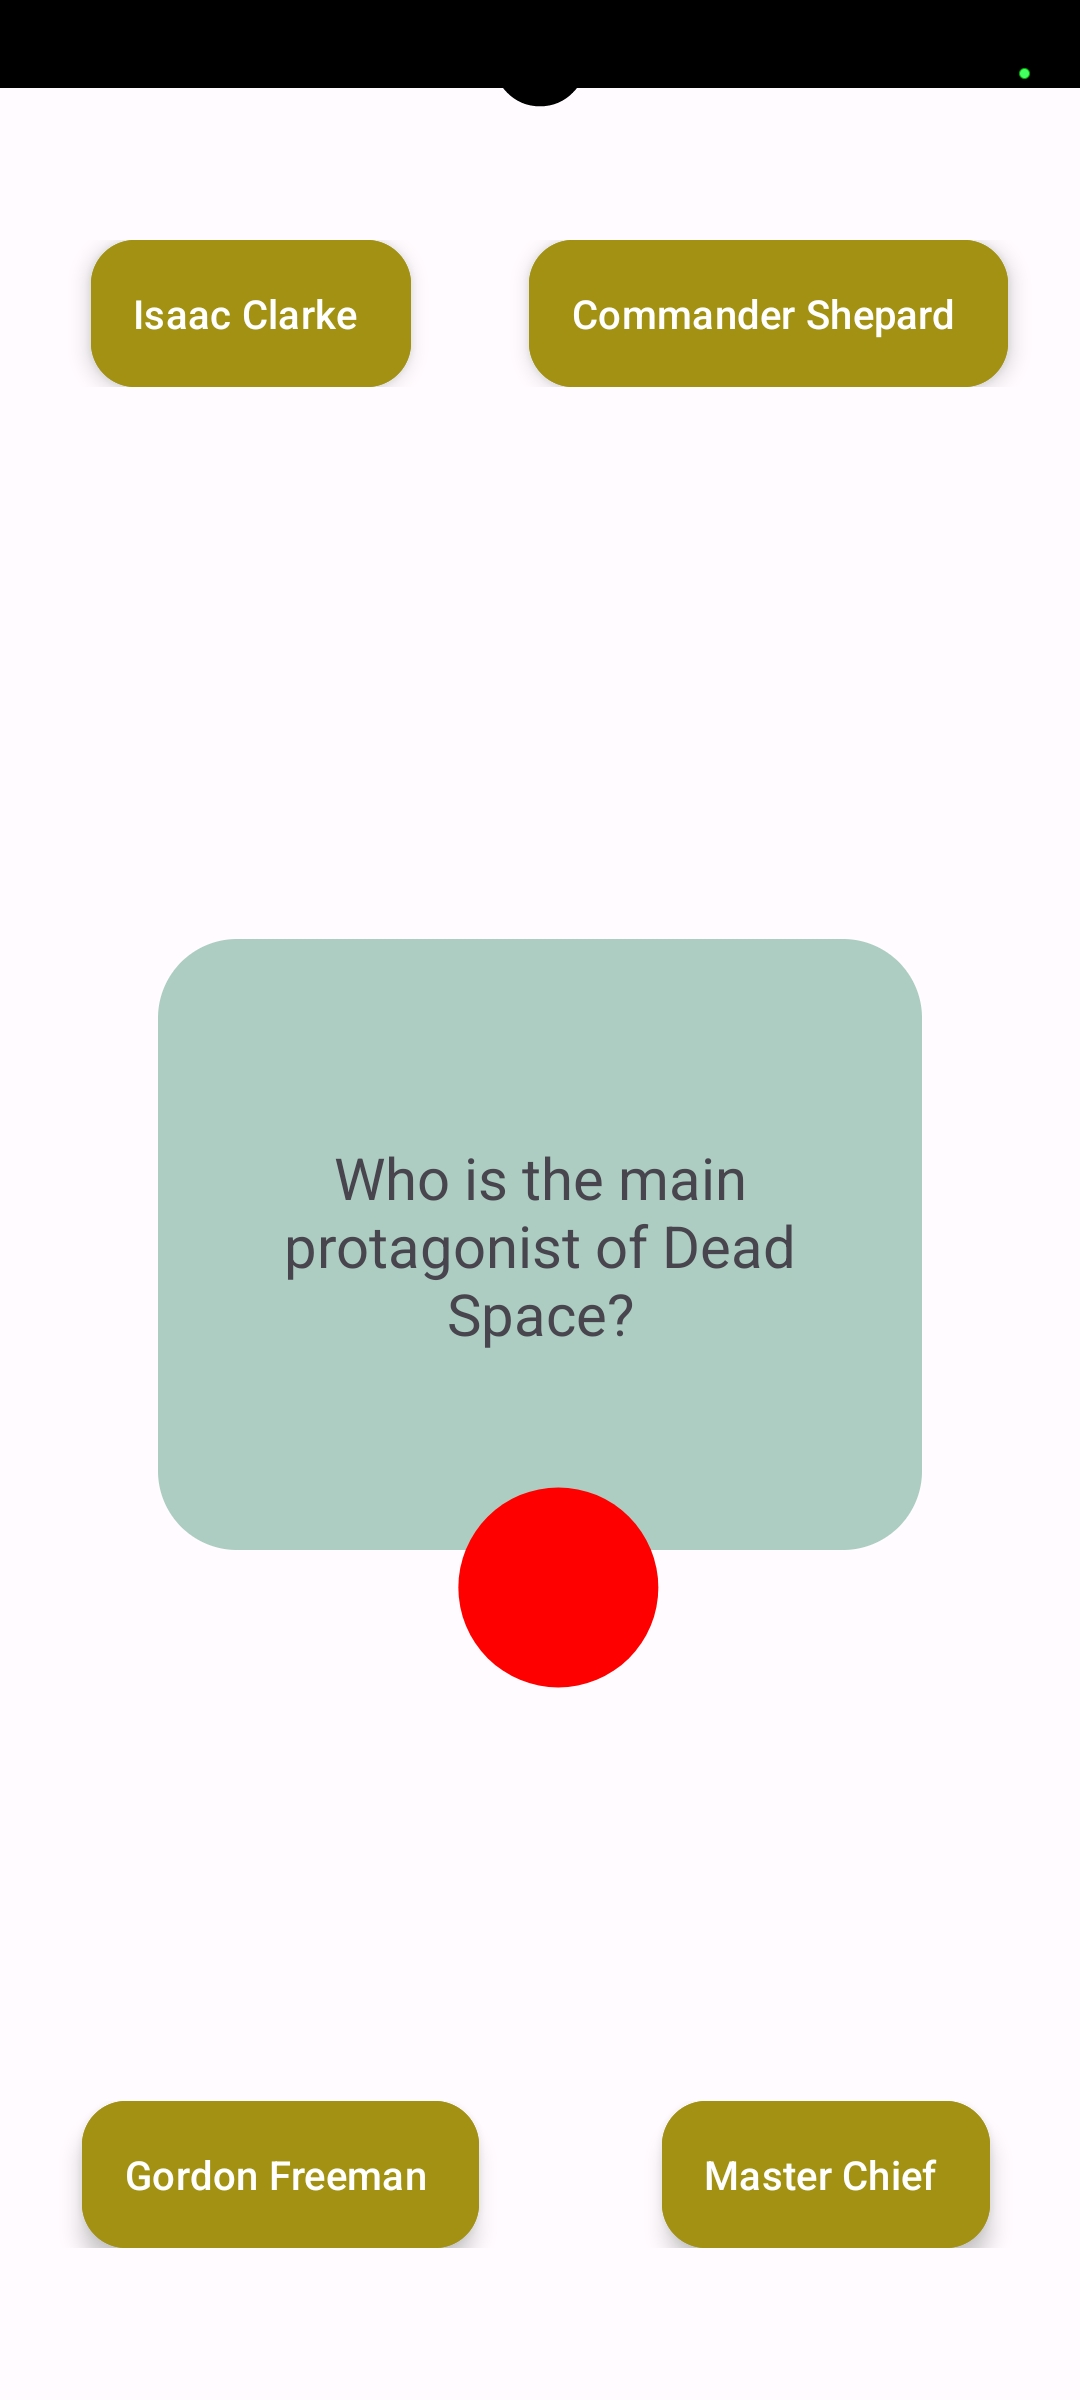
\includegraphics[scale=0.14]{ProgettoAndroid/Game/Images/CameraApp_Screen_quiz.jpg}
    \caption{Schermata Game}
    \label{fig:game}
\end{figure}